\section{Uso de la interfaz gráfica]} \label{GUI}

La interfaz gráfica de usuario (GUI) es la parte del programa que interactúa con el usuario.
Al ejecutar el programa, se abre una ventana que permite al usuario interactuar con el sistema CABRA.
La GUI se divide en cuatri secciones principales:
\begin{itemize}
    \item La barra de tareas, que permite configurar la conexión con el audiometro y especificar parámetros del
    estímulo.
    \item El panel de control, que permite al usuario configurar los parámetros de la audiometría.
    \item El panel de resultados, que muestra los resultados de la audiometría.
    \item La etiqueta de estado, que muestra el estado actual del sistema.
\end{itemize}

\begin{figure}[H]
    \centering
    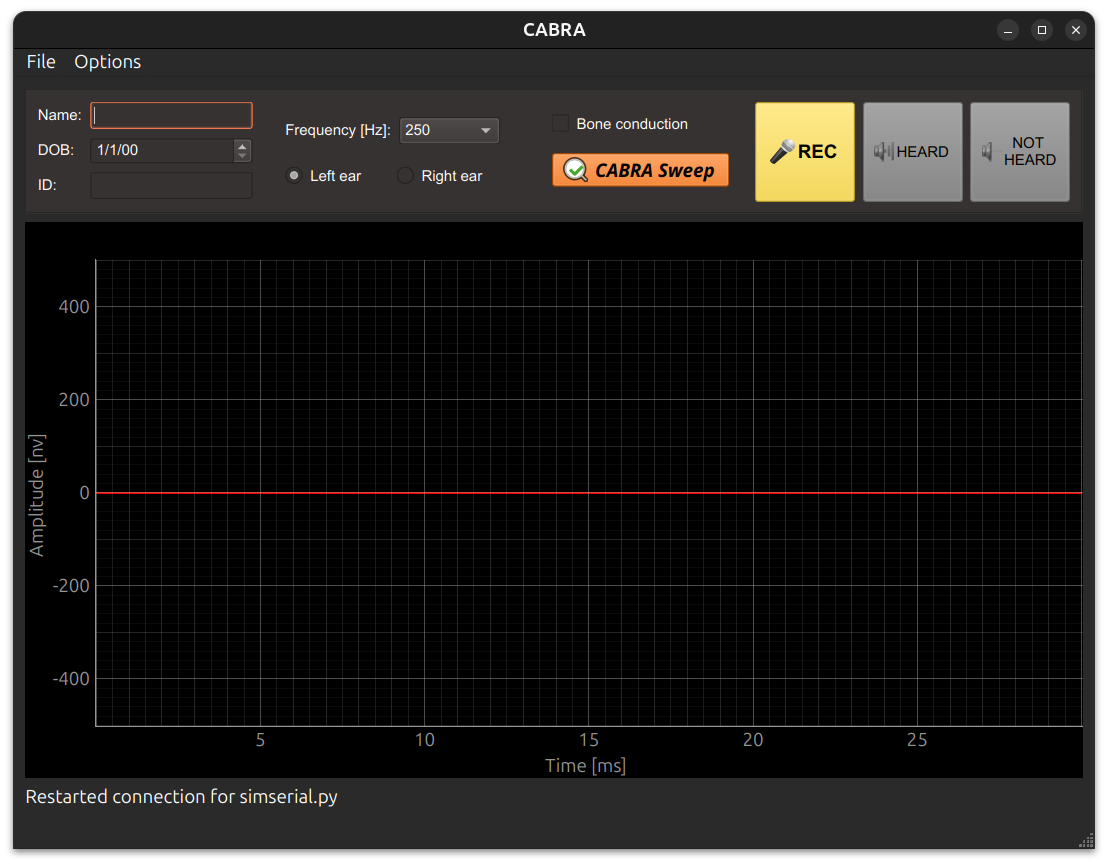
\includegraphics[width=0.8\textwidth]{figuras/gui_basic.png}
    \caption{Interfaz gráfica de usuario de CABRA}
    \label{fig:GUI_basic}
\end{figure}

Durante todo momento, se debe prestar particular atención a la etiqueta de estado, ya que informa al usuario sobre
el estado actual del sistema y sobre los próximos pasos a seguir.

\subsection{Verificación de la conexión con CABRA}

Al inicializar el programa, debería visualizarse en la etiqueta de estado el mensaje \textit{Connection established}.
Caso contrario, se abrirá una ventana emergente que indicando el error.

\begin{figure}[H]
    \centering
    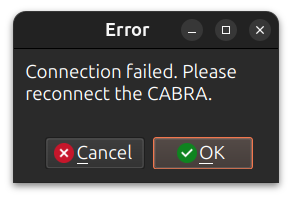
\includegraphics[width=0.4\textwidth]{figuras/connection_error_popup}
    \caption{Ventana emergente de error}
    \label{fig:GUI_conn_error}
\end{figure}

En caso de que se presente un error, se debe verificar que el audiometro esté conectado al puerto USB de la computadora.
Luego, indicar "OK" en la ventana emergente para cerrarla y volver a intentar la conexión.

\textit{Observación}: si se selecciona la opción "Cancel", la ventana emergente se cerrará, y el programa pasará
automáticamente a funcionar en modo de simulación.
La sección \ref{simulacion} describe el modo de simulación en detalle.

\subsection{Realización del estudio de audiometría}

Para realizar la audiometría, se deben configurar algunos parámetros de la prueba.
Estos parámetros se dividen en dos secciones: la información personal del paciente (nombre, fecha de nacimiento,
ID) y la configuración de la audiometría (selección de oído, selección de frecuencia, método de conducción).
Luego, existen dos maneras de llevar a cabo el estudio: forma manual y forma automática.
A continuación, se describen ambas formas.

\subsubsection{Forma manual} \label{manual}

La metodología manual de la audiometría consiste en seleccionar manualmente cada frecuencia y cada oído, indicando
el método de conducción utilizado.
Luego de haber configurado los parámetros, se debe presionar el botón "REC" para comenzar la prueba.
Al oprimir este botón, el programa reproducirá un estímulo auditivo según la configuración seleccionada, a una
amplitud inicial de 0 [dbHL]. Al finalizar el estímulo, se visualizará en pantalla el potencial evocado obtenido,
junto con la onda V detectada.
Entonces, se activarán los botones de "HEARD" y "NOT HEARD", para que el usuario indique si el paciente escuchó o no
el estímulo.
Prestando atención a la etiqueta de estado, notará que el sistema le indicará una sugerencia de diagnóstico:
mediante un algoritmo de análisis de señales, CABRA le indicará si la onda visualizada indica o no percepción sonora.
El usuario no está obligado a seguir esta sugerencia, pero se recomienda hacerlo en casos de duda.

Al indicar si el sonido fue perceptible o no, mediante los ya mencionados botones de "HEARD" y "NOT HEARD", CABRA
automáticamente generará un nuevo estímulo auditivo, con una amplitud mayor o menor, según corresponda.
Este proceso se repetirá hasta que se encuentra, automáticamente, el umbral auditivo del paciente.
En ese momento, se visualizará en pantalla en la etiqueta de estado el valor de dicho umbral.
Este valor quedará almacenado internamente, y se utilizará más adelante para visualizar el audiograma.


\begin{figure}[H]
    \centering
    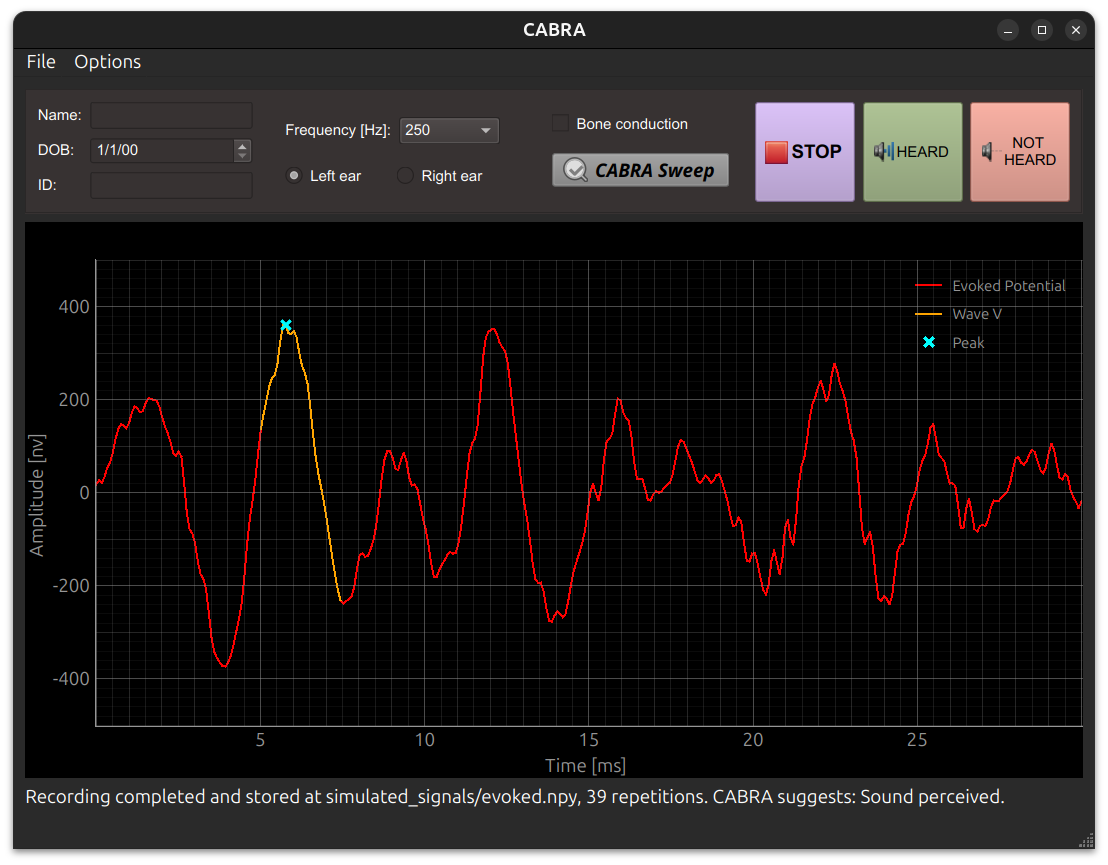
\includegraphics[width=0.8\textwidth]{figuras/cabra_gui_test_evoked}
    \caption{Interfaz gráfica de usuario de CABRA durante la realización de una audiometría}
    \label{fig:GUI_manual}
\end{figure}

Para continuar con el estudio, se debe realizar un barrido completo de todas las frecuencias y ambos oídos.
Al finalizar, se visualizará en pantalla el audiograma del paciente, y se almacenará en un archivo.

\begin{figure}[H]
    \centering
    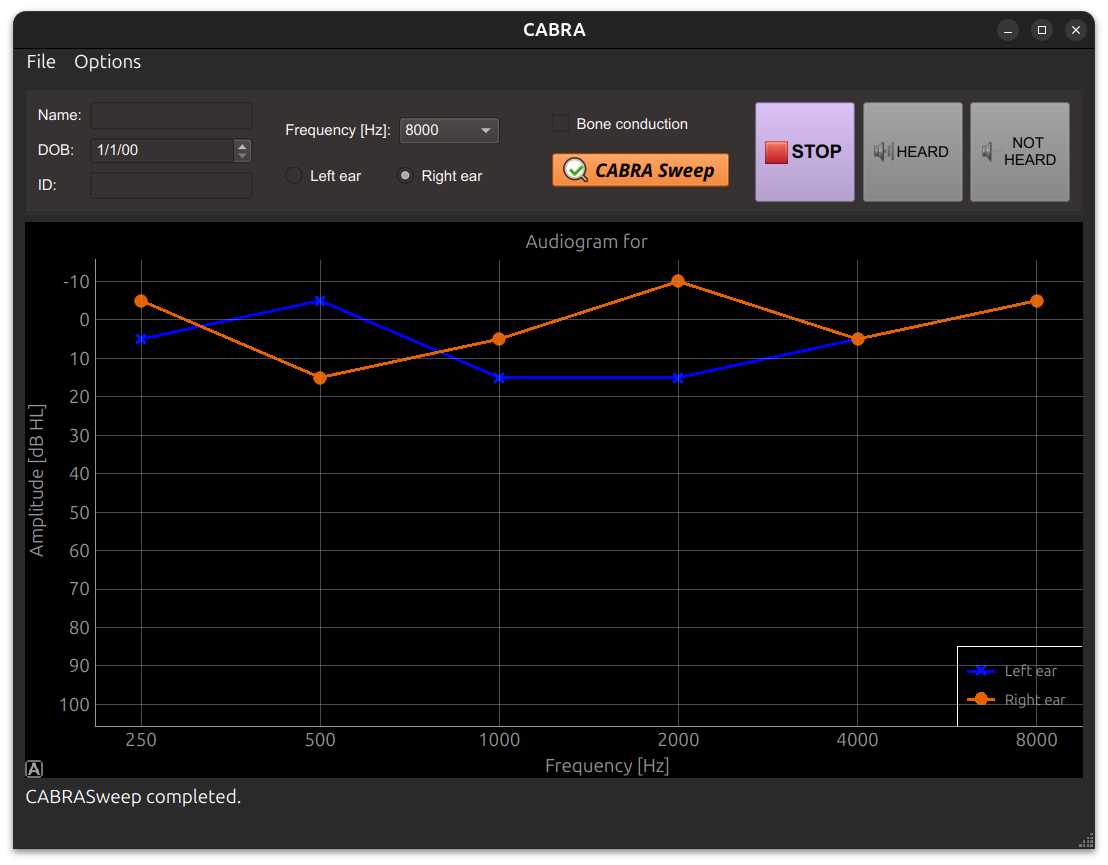
\includegraphics[width=0.8\textwidth]{figuras/GUI_audiogram}
    \caption{Interfaz gráfica de usuario de CABRA al finalizar una audiometría}
    \label{fig:GUI_audiogram}
\end{figure}


\subsubsection{Forma automática (CABRASweep)}

Realizar un barrido manual de todo el rando de frecuencias para ambos oídos puede ser tedioso y llevar mucho tiempo.
Además, es posible que el usuario cometa errores al seleccionar los parámetros, como ignorar una prueba o evaluar
dos veces las mismas condiciones.
Para evitar esto, CABRA cuenta con el botón \textit{CABRASweep}, que permite realizar un barrido automático de todas
las frecuencias y ambos oídos.
Al presionar este botón, el programa realizará automáticamente todas las pruebas, avanzando de frecuencia en
frecuencia.
El usuario, por su parte, sólo deberá indicar si el paciente escuchó o no cada estímulo, de la misma manera que se
describió en la sección anterior \ref{manual}.
Al finalizar, se visualizará en pantalla el audiograma del paciente, y se almacenará en un archivo.

\subsection{Ajuste de parámetros avanzados}

Los estímulos generados por CABRA son de la forma \textit{tone bursts}, que consisten en una onda senoidal de
frecuencia fija, con una duración de duración predeterminada, seguido de silencio.
Este estímulo se repite varias veces, y se promedian los resultados de cada medición para obtener un potencial evocado.
Por lo tanto, el estímulo generado se caracteriza por su frecuencia, duración del tono, duración del silencio, y
número de repeticiones.

A priori, desde el panel de control, sólo se puede elegir la frecuencia del sonido, y se toma por default una
duración del tono de 10 [ms], una duración total del ciclo de 30 [ms] (es decir: 10 [ms] de tono y 20 [ms] de
silencio), y 500 repeticiones.
Los valores de duraión del tono y del ciclo, así como el número de repeticiones, se pueden modificar mediante la
barra de herramientas, seleccionando "Options" y luego "Tone burst setup".
Esto abrirá una ventana emergente que permite modificar estos parámetros.

\begin{figure}[H]
    \centering
    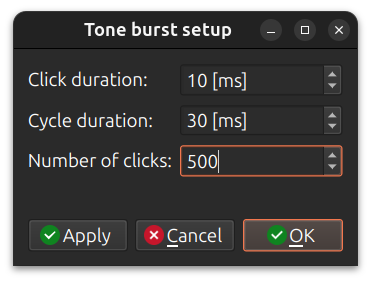
\includegraphics[width=0.4\textwidth]{figuras/tone_bursts_setup}
    \caption{Ventana emergente de configuración de los parámetros del tono}
    \label{fig:GUI_tone_burst_setup}
\end{figure}

\subsection{Simulación} \label{simulacion}

Para facilitar la utilización del programa, CABRA cuenta con un modo de simulación.
Este modo permite al usuario familiarizarse con la interfaz gráfica y con los procedimientos de la audiometría, sin
la necesidad de contar con un audiometro conectado ni con un paciente.
Para activarlo, desde la barra de herramientas, seleccionar "Options", luego entrar al menú "Mode..." y seleccionar "
Simulator".
Para volver al modo original, seleccionar desde el mismo menú la opción "CABRA [default]".

